\documentclass[a4paper,12pt]{article}

\usepackage{fontspec}
\setmainfont{TeX Gyre Termes}
\usepackage{xeCJK}
\setCJKmainfont{Noto Serif CJK SC}
\setCJKsansfont{Noto Sans CJK SC}
\setCJKmonofont{Noto Sans CJK SC}

\usepackage{geometry}
\geometry{margin=2.5cm}
\usepackage{amsmath,amssymb,mathtools}
\usepackage{graphicx}
\usepackage{float}
\usepackage{booktabs}
\usepackage{array}
\usepackage{enumitem}
\usepackage{xurl}
\usepackage[colorlinks=true,linkcolor=blue,urlcolor=blue,citecolor=blue]{hyperref}
\usepackage{bookmark}
\usepackage{tikz}
\usetikzlibrary{shapes.geometric, arrows.meta, positioning}

\graphicspath{{figures/}}
\setlist[itemize]{leftmargin=2em}
\setlist[enumerate]{leftmargin=2em}
\linespread{1.12}

\DeclareMathOperator{\softmax}{softmax}
\DeclareMathOperator{\RMS}{RMS}
\DeclareMathOperator{\LN}{LN}
\DeclareMathOperator{\BN}{BN}

\title{Vision-Language Models from Scratch 阅读笔记}
\author{Yuyue}
\date{\today}

\begin{document}
\maketitle

\noindent 代码学习来源：
\url{https://www.youtube.com/watch?v=vAmKB7iPkWw&t=1431s}

\tableofcontents
\newpage

\section{整体脉络}

本文整理从零实现视觉语言模型时需要理解的几个核心模块：视觉编码器如何把图片变成 token，Transformer 如何通过 self-attention 让 token 互相交换信息，语言模型在推理时如何利用 KV cache、Grouped Query Attention 和位置编码高效生成下一个 token。

视觉语言模型通常可以被拆成三部分：
\begin{enumerate}
    \item 视觉编码器：把图片切成 patch，并把每个 patch 映射成一个向量 token。
    \item 投影或对齐模块：把视觉 token 对齐到语言模型可以接收的 hidden size。
    \item 语言模型：把图像 token 和文本 token 一起作为上下文，持续预测下一个 token。
\end{enumerate}

\begin{figure}[H]
    \centering
    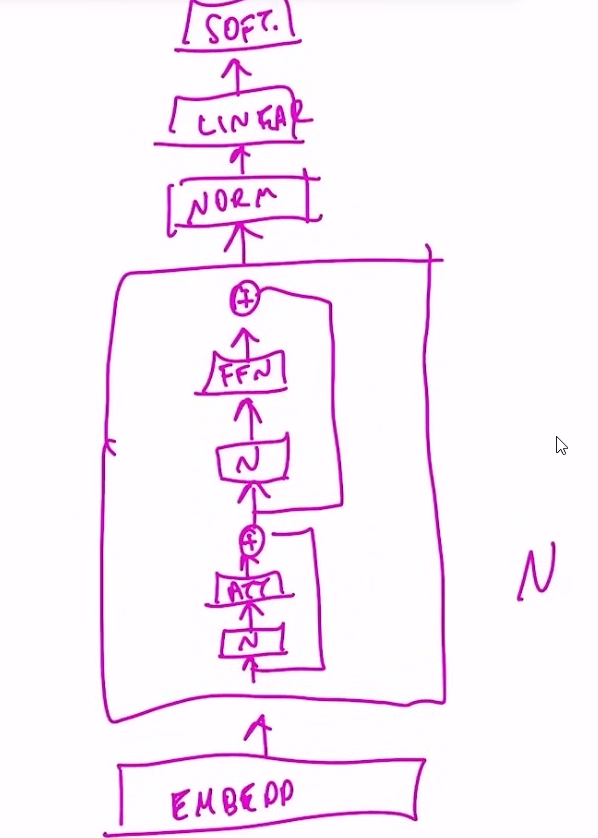
\includegraphics[width=0.42\textwidth]{架构图 .png}
    \caption{语言模型 Transformer 块的整体数据流}
\end{figure}

\section{SigLIP 与对比学习}

\subsection{Softmax 的数值稳定性}

Softmax 定义为
\[
    \softmax(z_i)=\frac{e^{z_i}}{\sum_j e^{z_j}}.
\]
当 $z_i$ 很大或很小时，直接计算指数容易出现数值不稳定。常用的稳定写法是减去最大值：
\[
    \softmax(z_i)=
    \frac{e^{z_i-\max_j z_j}}
    {\sum_j e^{z_j-\max_j z_j}}.
\]
这样不会改变 softmax 的输出比例，但可以避免指数溢出。

\subsection{为什么 SigLIP 使用 Sigmoid Loss}

在 CLIP 一类对比学习中，图像和文本会形成一个相似度矩阵，softmax 通常需要在整行或整列上归一化。这会让每个样本依赖同一个 batch 中的其他样本，并且在超大 batch 训练时带来通信和并行化压力。

SigLIP 的思路是把图文匹配改写成独立的二分类问题，用 sigmoid loss 判断一对图像和文本是否匹配。Sigmoid 定义为
\[
    \sigma(z)=\frac{1}{1+e^{-z}}.
\]
每一对样本的损失可以相对独立地计算，因此更适合大 batch 和分布式训练。

\subsection{对比式视觉编码器的目标}

对比学习的目标是让匹配的图像 embedding 和文本 embedding 更接近，让不匹配的 pair 更远。这样训练出来的视觉编码器不只是记住类别，而是学习能和语言语义对齐的图像表示。后续在图像问答、图像描述、视觉推理等任务中，语言模型就可以把视觉 token 当作上下文来使用。

\section{Vision Transformer}

\subsection{从图片到 Patch Token}

Vision Transformer 首先把图片切成固定大小的 patch。实现时常用一个卷积层完成 patch embedding：令卷积核大小等于 patch size，stride 也等于 patch size，这样每个卷积输出位置对应一个 patch。然后把二维 patch 序列 flatten 成一维 token 序列。

\begin{figure}[H]
    \centering
    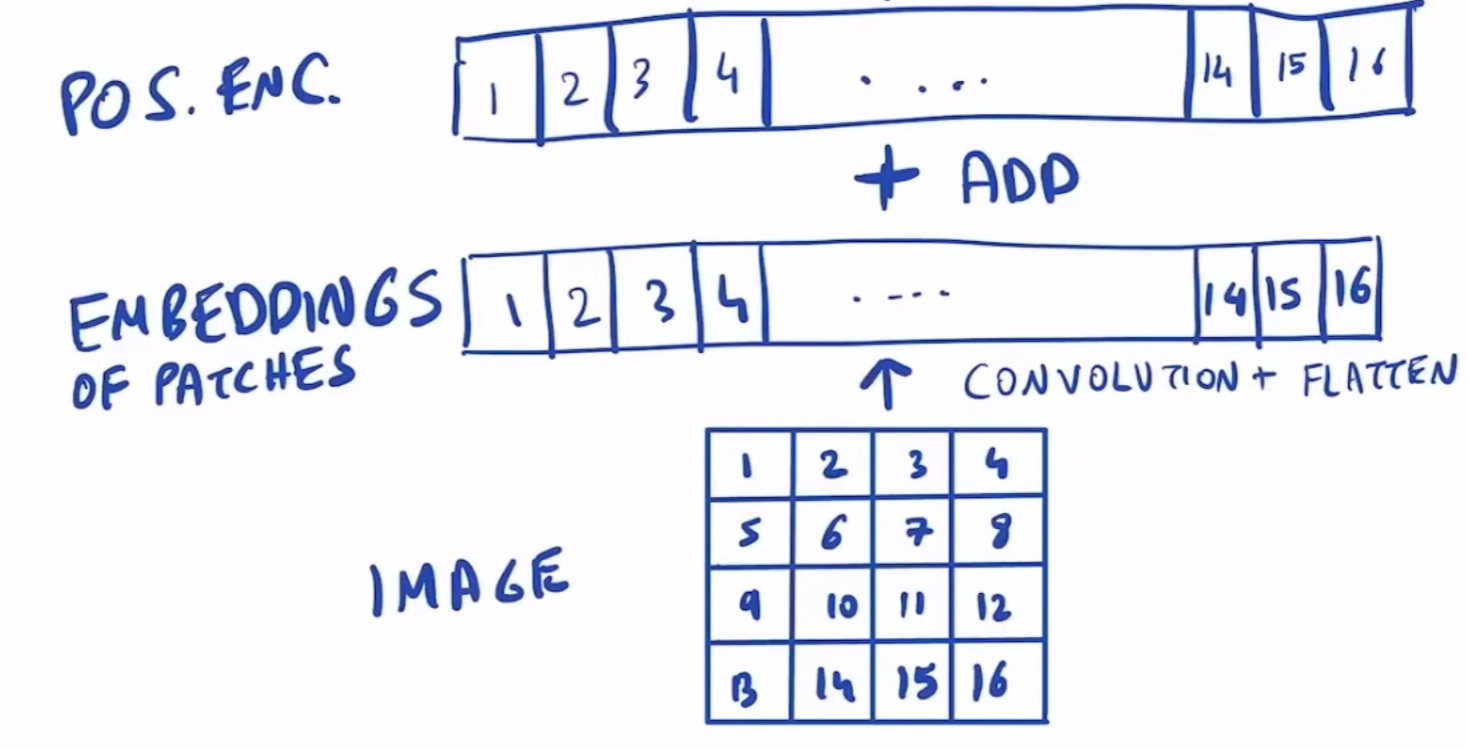
\includegraphics[width=0.85\textwidth]{vision_transformer_explaination.png}
    \caption{Vision Transformer 中图片 patch、patch embedding 和位置编码的关系}
\end{figure}

如果一张图片被切成 $N$ 个 patch，每个 patch embedding 的维度是 $D$，那么进入 Transformer 前的张量可以看成
\[
    X\in \mathbb{R}^{N\times D}.
\]
每一行是一个 patch token，每一列是该 token 的一个特征维度。

\subsection{位置编码}

Transformer 本身不包含序列顺序信息，因此需要位置编码。对于 ViT，位置编码通常在 patch embedding 进入 Transformer 之前加入：
\[
    X_{\text{input}} = X_{\text{patch}} + E_{\text{pos}}.
\]
这里的 $E_{\text{pos}}$ 可以是可学习参数。它不一定要由 $\sin$ 或 $\cos$ 固定生成，模型可以通过训练自己学习有用的位置模式。

\begin{figure}[H]
    \centering
    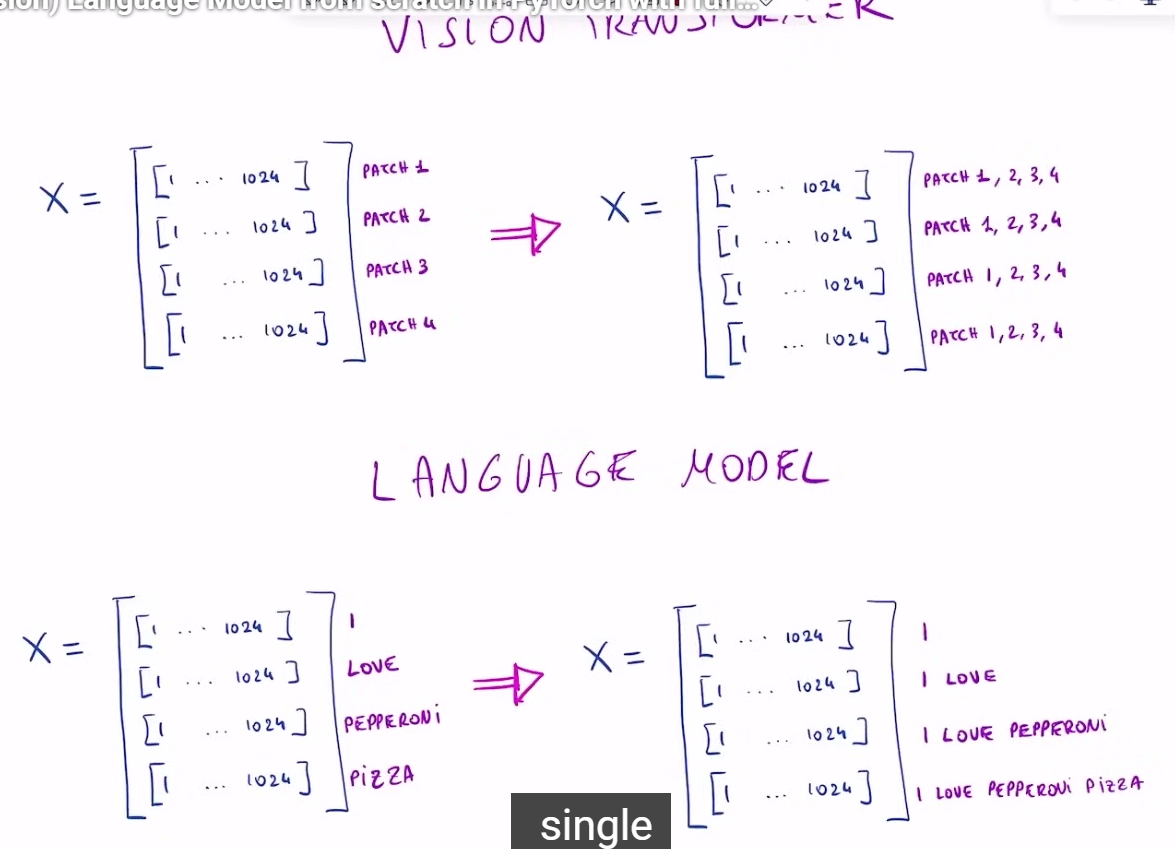
\includegraphics[width=0.85\textwidth]{vision transformer and normal transformer.png}
    \caption{Vision Transformer 与语言模型 Transformer 的输入上下文差异}
\end{figure}

ViT 的 self-attention 通常不需要 causal mask，因为图像中的每个 patch 可以同时看见其他 patch；语言模型在训练和生成时则需要避免当前位置看到未来 token。

\subsection{Transformer Encoder Layer}

ViT encoder 由多个 Transformer encoder layer 堆叠而成。每一层通常包含：
\begin{itemize}
    \item LayerNorm 或 RMSNorm：稳定每一层的输入分布。
    \item Multi-Head Self-Attention：让不同 patch 之间交换信息。
    \item MLP/Feed Forward Network：对每个 token 独立做非线性变换。
    \item Residual Connection：缓解深层网络训练中的梯度传播问题。
\end{itemize}

\begin{figure}[H]
    \centering
    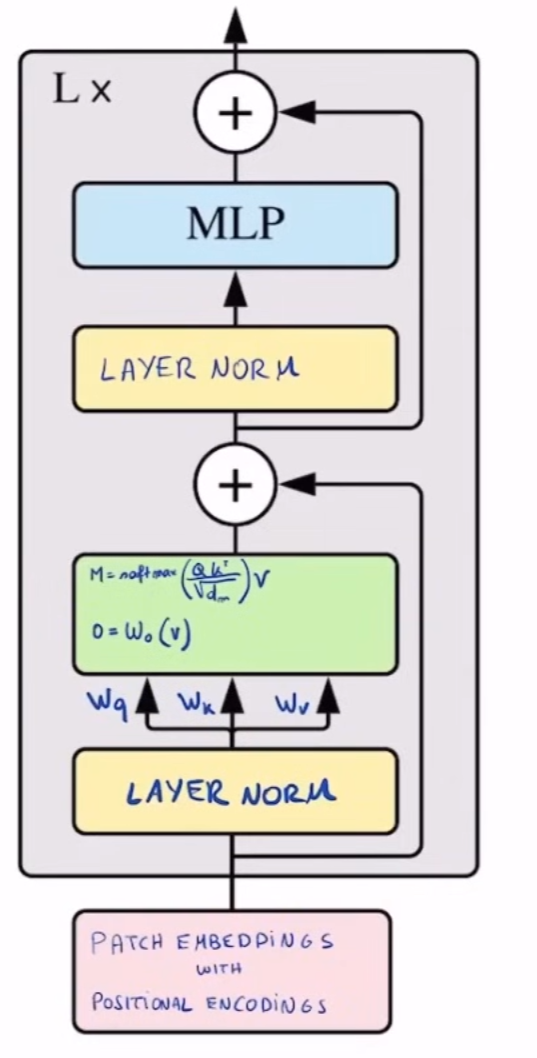
\includegraphics[width=0.50\textwidth]{encoder_layer.png}
    \caption{Transformer Encoder Layer 的基本结构}
\end{figure}

Self-attention 的输出形状和输入形状相同，但每个 token 的 embedding 已经包含其他 token 的上下文信息。也就是说，输出不再只是某个 patch 自己的信息，而是该 patch 和整张图片其他 patch 交互后的表示。

\section{Self-Attention 与 Multi-Head Attention}

\subsection{\texorpdfstring{从 $X$ 得到 $Q,K,V$}{从 X 得到 Q,K,V}}

Self-attention 首先用三个线性变换把输入 $X$ 映射成 query、key、value：
\[
    Q=XW_q,\qquad K=XW_k,\qquad V=XW_v.
\]
例如，当 sequence length 为 $4$、hidden size 为 $1024$、head 数为 $8$、每个 head 的维度为 $128$ 时，有
\[
    Q=(4,1024)\times(1024,8,128)=(4,8,128).
\]
其中 $8\times128=1024$，所以多头拆分不会改变总 hidden size，只是把一个大的向量分成多个 head。

\begin{figure}[H]
    \centering
    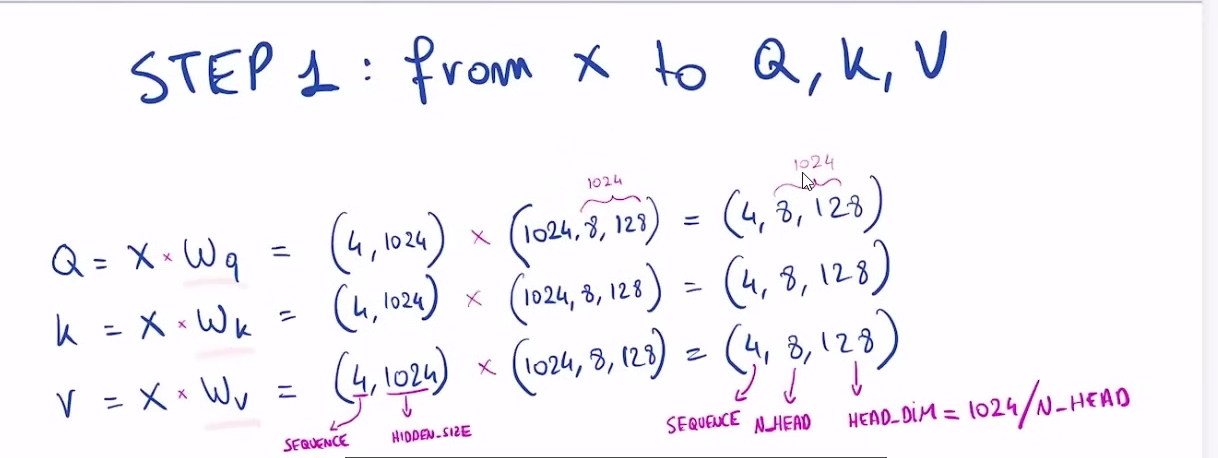
\includegraphics[width=0.85\textwidth]{QKV_calculate.png}
    \caption{由输入 $X$ 计算 $Q,K,V$ 的形状变化}
\end{figure}

\begin{figure}[H]
    \centering
    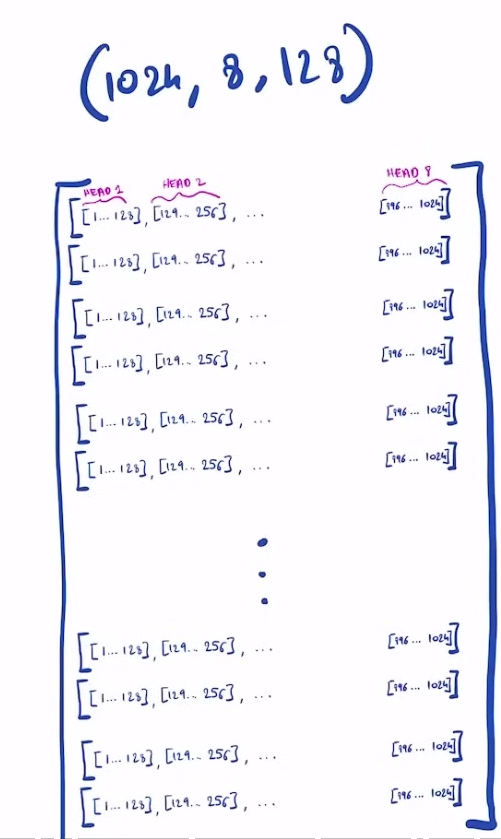
\includegraphics[width=0.85\textwidth]{W_q.png}
    \caption{$W_q$ 的多头参数组织方式}
\end{figure}

每个 head 只处理 $128$ 维子空间。不同 head 可以关注 embedding 中不同的语义子空间，并且各个 head 的注意力计算可以并行完成。

\subsection{转置与 Head 维度}

为了方便并行计算，通常会把张量从
\[
    (\text{seq}, \text{n\_heads}, \text{head\_dim})
\]
转置成
\[
    (\text{n\_heads}, \text{seq}, \text{head\_dim}).
\]
这样每个 head 都可以被看成一个独立的注意力问题。

\begin{figure}[H]
    \centering
    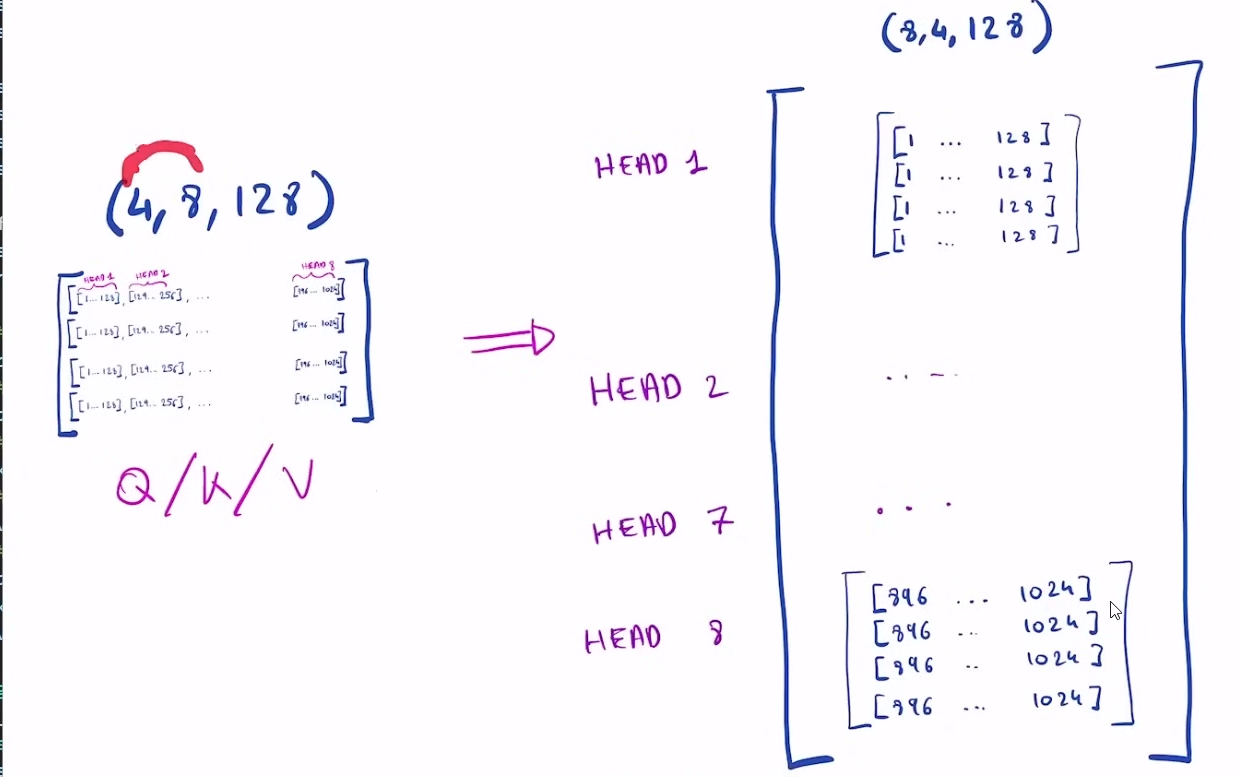
\includegraphics[width=1.0\textwidth]{data_transpose.png}
    \caption{为了按 head 并行计算而进行的数据转置}
\end{figure}

\subsection{Attention Score}

单个 head 中，attention score 由 query 和 key 的点积得到：
\[
    S=\frac{QK^\top}{\sqrt{d_{\text{head}}}}.
\]
除以 $\sqrt{d_{\text{head}}}$ 是为了控制点积数值规模，避免维度变大后 logits 过大，导致 softmax 过于尖锐、训练不稳定。

\begin{figure}[H]
    \centering
    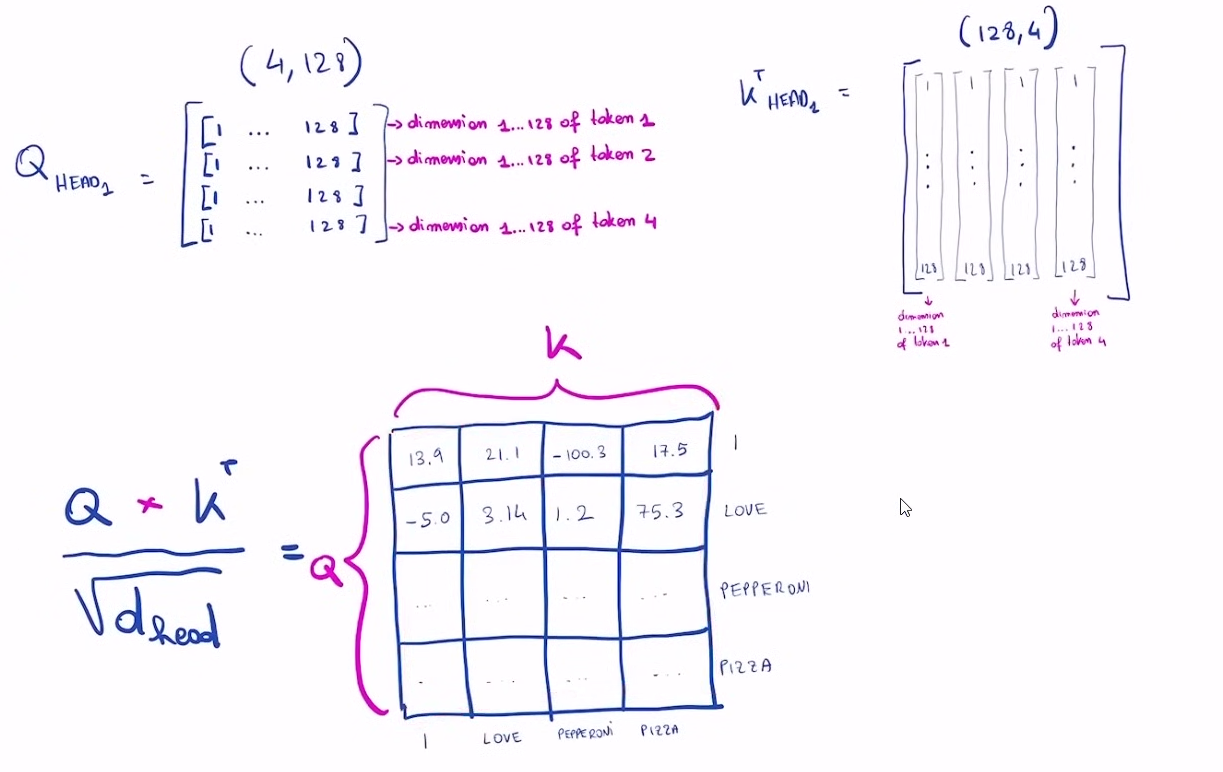
\includegraphics[width=0.85\textwidth]{attention_data.png}
    \caption{Attention score 矩阵的直观含义}
\end{figure}

对 score 做 softmax 后得到 attention weights：
\[
    A=\softmax\left(\frac{QK^\top}{\sqrt{d_{\text{head}}}}\right).
\]
矩阵 $A$ 的第 $i$ 行表示第 $i$ 个 token 对所有 token 的关注程度。

\subsection{Attention Output}

Attention 输出通过权重矩阵乘以 value 得到：
\[
    O=AV.
\]
例如：
\[
    A(4\times4)\times V(4\times128)=O(4\times128).
\]
这本质上是对所有 value row 做加权求和。某个输出 token 的表示由它对其他 token 的注意力权重决定，因此 attention 可以把上下文信息混入当前 token。

多个 head 的输出会被 concat 回 hidden size，然后再经过输出投影 $W_o$：
\[
    \operatorname{MHA}(X)=\operatorname{Concat}(O_1,\ldots,O_h)W_o.
\]
$W_o$ 的作用不是简单拼接，而是混合不同 head 的结果，让不同子空间的信息重新交互。

\section{Normalization}

\subsection{为什么需要 Normalization}

如果一层输入分布变化很大，它的输出、loss、gradient 和权重更新也会跟着大幅变化，训练会变慢甚至不稳定。

\begin{figure}[H]
    \centering
    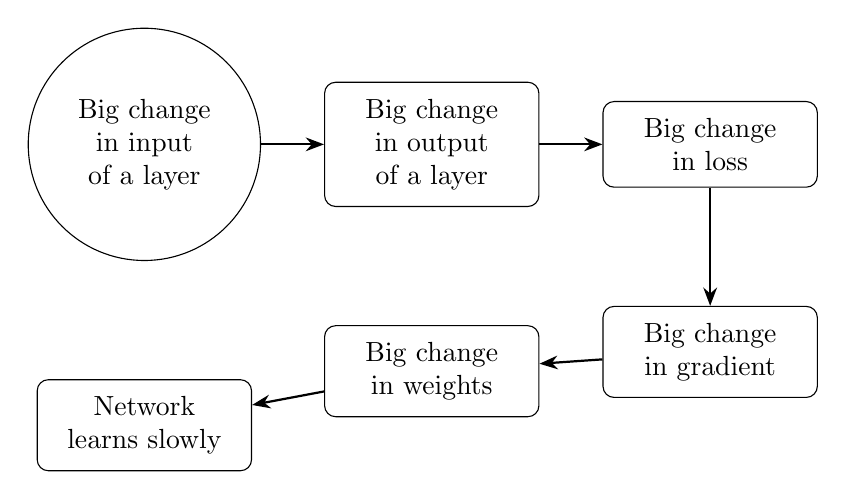
\begin{tikzpicture}[
        node distance=1.5cm and 0.8cm,
        box/.style={draw, rounded corners, text width=2.3cm, align=center, inner sep=6pt},
        circled/.style={draw, circle, text width=2.3cm, align=center, inner sep=4pt},
        arr/.style={-{Stealth}, thick}
        ]
        \node[circled] (A) {Big change in input of a layer};
        \node[box, right=of A] (B) {Big change in output of a layer};
        \node[box, right=of B] (C) {Big change in loss};
        \node[box, below=1.5cm of C] (D) {Big change in gradient};
        \node[box, below=1.5cm of B] (E) {Big change in weights};
        \node[box, below=1.5cm of A] (F) {Network learns slowly};
        \draw[arr] (A) -- (B);
        \draw[arr] (B) -- (C);
        \draw[arr] (C) -- (D);
        \draw[arr] (D) -- (E);
        \draw[arr] (E) -- (F);
    \end{tikzpicture}
    \caption{输入分布变化会逐层放大，Normalization 可以稳定训练}
\end{figure}

\subsection{BatchNorm 与 LayerNorm}

BatchNorm 通常沿 batch 维度统计均值和方差：
\[
    \BN(x)=\gamma\frac{x-\mu}{\sqrt{\sigma^2+\epsilon}}+\beta.
\]
它对 batch size 有依赖，batch 很小时统计量可能不稳定。

LayerNorm 则对单个 token 的 feature 维度做归一化：
\[
    \LN(x)=\gamma\frac{x-\mu}{\sqrt{\sigma^2+\epsilon}}+\beta.
\]
它不依赖 batch size，因此更适合 Transformer 中不同长度、不同 batch 的序列建模。

\subsection{RMSNorm}

RMSNorm 只使用均方根做缩放，不减去均值：
\[
    \RMS(x)=\sqrt{\frac{1}{d}\sum_{i=1}^{d}x_i^2+\epsilon},
    \qquad
    \operatorname{RMSNorm}(x)=\frac{x}{\RMS(x)}\odot g.
\]
其中 $g$ 是可学习缩放参数。相比 LayerNorm，RMSNorm 计算更简单，也被很多语言模型采用。

\begin{figure}[H]
    \centering
    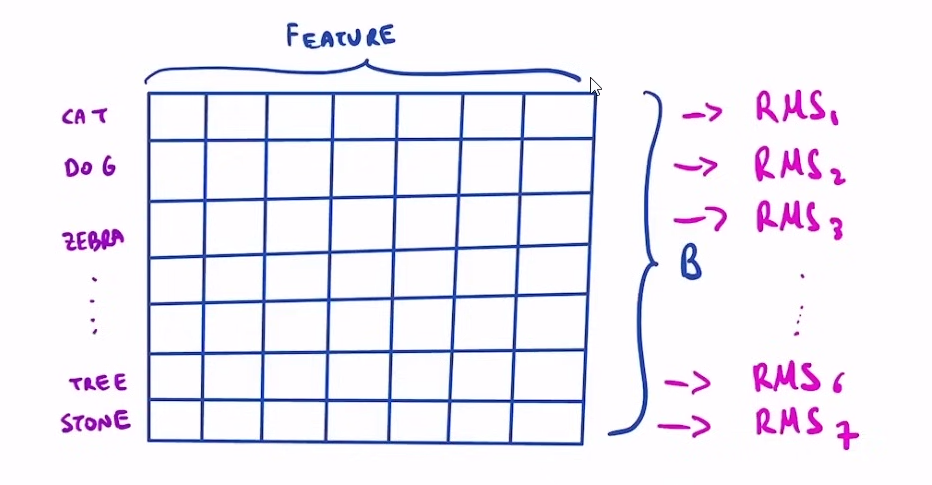
\includegraphics[width=0.80\textwidth]{RMS.png}
    \caption{RMSNorm 在 token feature 维度上的归一化方式}
\end{figure}

\section{KV Cache 与高效推理}

\subsection{自回归生成中的重复计算}

语言模型生成文本时，每一步只需要预测下一个 token。假设当前 prompt 是 ``I LOVE''，模型会先根据上下文预测下一个 token；得到新 token 后再把它追加到序列中，继续预测。

如果每一步都重新计算完整前缀的 $K$ 和 $V$，会产生大量重复计算。KV cache 的核心思想是：历史 token 的 $K,V$ 一旦算出就缓存下来，下一步只为新 token 计算新的 $Q,K,V$，并把新的 $K,V$ append 到 cache。

\begin{figure}[H]
    \centering
    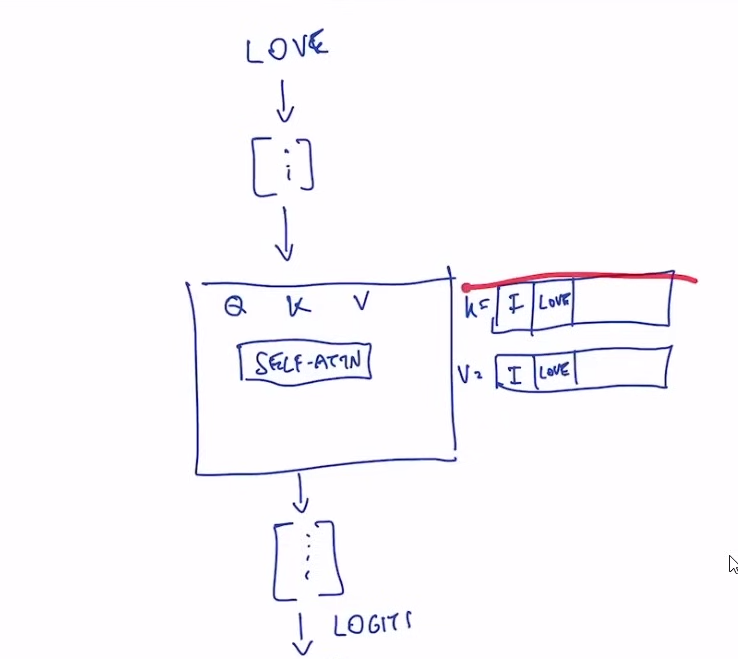
\includegraphics[width=0.85\textwidth]{kvcache.png}
    \caption{KV cache 在自回归推理中的使用方式}
\end{figure}

Prefill 阶段会一次性处理完整 prompt，并写入 cache；decode 阶段每次只输入最新 token。当前 token 的 query 会和 cache 中所有历史 key 做 attention，再用历史 value 得到当前 token 的上下文化表示。

\subsection{Grouped Query Attention}

Multi-Head Attention 中，通常 $Q,K,V$ 都有相同数量的 head。例如 hidden size 为 $1024$、head 数为 $8$ 时，每个 head 维度为 $128$：
\[
    \text{Head}_1=[1,\ldots,128],\quad
    \text{Head}_2=[129,\ldots,256],\quad
    \ldots,\quad
    \text{Head}_8=[897,\ldots,1024].
\]

推理时最大的瓶颈往往不是矩阵乘法本身，而是从显存读取 KV cache。GPU 的 HBM 容量大但读写代价高，片上/local memory 容量小但速度快；很多时候计算比搬运数据更便宜。

Grouped Query Attention（GQA）让多个 query head 共享同一组 key/value head。例如 8 个 query head 可以分成若干组，每组共享一个 key head 和 value head。这样可以减少 KV cache 的大小和显存带宽需求。

实现时常见做法是先保存较少数量的 key/value head，在 attention 计算前通过 repeat 或 expand 让它们在形状上匹配 query head 数：
\[
    n_{\text{kv\_heads}} < n_{\text{q\_heads}},\qquad
    K,V \rightarrow \operatorname{repeat\_kv}(K,V).
\]
这种方法用少量额外计算换取更少的数据读取。代价是不同 query head 共享同一组 $K,V$，表达能力可能略弱于完整 MHA，但推理速度和显存占用通常更好。

\subsection{Gradient Checkpointing 的权衡}

手写笔记中提到的 ``redo the computation rather than copy them'' 对应一种常见思想：用重新计算换显存或数据搬运。Gradient checkpointing 在训练时不保存所有中间激活，而是在反向传播需要时重新计算部分前向结果。它牺牲一部分计算量，换取更低显存占用。

\section{位置编码与 RoPE}

\subsection{绝对位置与相对位置}

普通位置 embedding 是在 Transformer 入口处直接加到 token embedding 上。它告诉模型每个 token 处在序列的哪个绝对位置。

语言模型还需要表达相对位置：第 $m$ 个 token 和第 $n$ 个 token 的关系，应该依赖 $m-n$。一个理想形式是
\[
    \langle f_q(x_m,m), f_k(x_n,n)\rangle
    =g(x_m,x_n,m-n).
\]
也就是说，query 和 key 的点积不仅由 token 内容决定，也由它们之间的相对距离决定。

\subsection{RoPE 的旋转形式}

RoPE（Rotary Position Embedding）通过旋转 query 和 key 的二维子空间来注入位置。对一对维度，可以写成
\[
    R_{m\theta}
    =
    \begin{bmatrix}
        \cos m\theta & -\sin m\theta \\
        \sin m\theta & \cos m\theta
    \end{bmatrix}.
\]
对于更高维的 hidden vector，会把相邻的两个维度作为一组，使用不同频率的 $\theta_i$：
\[
    \theta_i = 10000^{-2i/d},\qquad i\in\left[0,\frac{d}{2}\right).
\]

高效实现通常不显式构造大旋转矩阵，而是使用逐元素乘法：
\[
    \operatorname{RoPE}(x,m)
    =
    x\odot \cos(m\theta)
    +
    \operatorname{rotate\_half}(x)\odot \sin(m\theta).
\]
其中
\[
    \operatorname{rotate\_half}([x_1,x_2,x_3,x_4,\ldots])
    =
    [-x_2,x_1,-x_4,x_3,\ldots].
\]

RoPE 被加在 $Q$ 和 $K$ 上，而不是 $V$ 上，因为 attention score 来自 $QK^\top$。这样 score 会自然包含相对位置信息。

\section{Token 生成与采样}

\subsection{Logits 到下一个 Token}

语言模型最后一层输出 vocabulary size 维度的 logits：
\[
    z\in\mathbb{R}^{|\mathcal{V}|}.
\]
每个 logit 对应词表中一个 token 的分数。最简单的 greedy decoding 直接取最大值：
\[
    y=\arg\max_i z_i.
\]
这种方法稳定但容易缺少多样性。

\subsection{\texorpdfstring{Top-$p$ Sampling}{Top-p Sampling}}

另一种做法是先把 logits 转成概率：
\[
    p_i=\softmax(z_i),
\]
再按概率从高到低排序，保留累计概率达到阈值 $p$ 的最小 token 集合，然后只在这个集合里采样。这就是 top-$p$ sampling，也叫 nucleus sampling。

Top-$p$ 的作用是过滤掉尾部低概率 token，减少明显不合理的输出，同时保留一定随机性。

\subsection{Temperature}

Temperature 通过缩放 logits 控制分布尖锐程度：
\[
    p_i=\softmax\left(\frac{z_i}{T}\right).
\]
当 $T<1$ 时，logits 之间的差距被放大，模型更倾向于高分 token；当 $T>1$ 时，分布变平，更多 token 有机会被采样，输出更有多样性但也更容易引入噪声。

\section{总结}

视觉语言模型的关键是把图像 patch token 和文本 token 放到统一的 Transformer 语义空间中。ViT 负责把图片转成上下文化视觉表示；self-attention 通过 $Q,K,V$ 的点积和加权求和建模 token 之间的关系；Normalization 保证深层网络稳定训练；KV cache、GQA 和 RoPE 则是语言模型高效推理不可缺少的工程与建模技巧。

\end{document}
